\documentclass{article}
\usepackage[T1]{fontenc}
\usepackage{lmodern}
\usepackage{graphicx}
\usepackage{amsmath,amssymb}
\usepackage[a4paper,margin=2cm]{geometry}
\usepackage[absolute,overlay]{textpos}
\setlength{\TPHorizModule}{1mm}
\setlength{\TPVertModule}{1mm}
\usepackage[indonesian]{babel}
\usepackage{hyperref}
\setlength{\emergencystretch}{2em}
% unit: Halaman 12

\begin{document}

% === Halaman 12 (python/native) ===

“Aman” artinya:

1. Terjaga kerahasiaannya (confidentiality)

12

2. Terjaga keasliannya (data integrity)

Pesan asli

Pesan sudah diubah

Suhu di luar 33 

derajat celcius

Suhu di luar 32 

derajat celcius

Pesan asli

Pesan sudah diubah

% deskripsi: gambar native xref 71
\noindent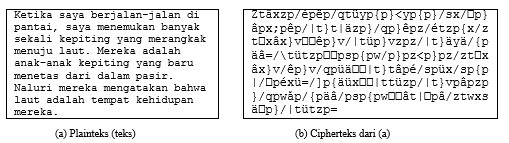
\includegraphics[width=0.85\textwidth]{../../images/python/page_012_img_01.png}

% deskripsi: gambar native xref 72
\noindent
\includegraphics[width=0.85\textwidth]{../../images/python/page_012_img_02.jpeg}

% deskripsi: gambar native xref 73
\noindent
\includegraphics[width=0.85\textwidth]{../../images/python/page_012_img_03.jpeg}

\end{document}
